% Source: Code/radar-scene-augmentation/echo-trail-generator/docs/config_reference.tex
% Description: Comparison of decay curves.  \texttt{linear

\documentclass[border=4pt]{standalone}
\usepackage{amsmath}
\usepackage{pgfplots}
\usepackage{tikz}
\usepackage{xcolor}
\pgfplotsset{compat=1.18}
\usetikzlibrary{arrows.meta, positioning, calc, shapes.geometric}

\definecolor{Garnet}{HTML}{73000A}
\definecolor{Black}{HTML}{000000}
\definecolor{White}{HTML}{FFFFFF}
\definecolor{NinetyBlack}{HTML}{363636}
\definecolor{SeventyBlack}{HTML}{5C5C5C}
\definecolor{FiftyBlack}{HTML}{A2A2A2}
\definecolor{ThirtyBlack}{HTML}{C7C7C7}
\definecolor{TenBlack}{HTML}{ECECEC}
\definecolor{WarmGrey}{HTML}{676156}
\definecolor{Sandstorm}{HTML}{FFF2E3}
\definecolor{Rose}{HTML}{CC2E40}
\definecolor{Atlantic}{HTML}{466A9F}
\definecolor{Congaree}{HTML}{1F414D}
\definecolor{Horseshoe}{HTML}{65780B}
\definecolor{Grass}{HTML}{CED318}
\definecolor{Honeycomb}{HTML}{A49137}


\tikzset{every node/.append style={rounded corners=0pt}}

\begin{document}
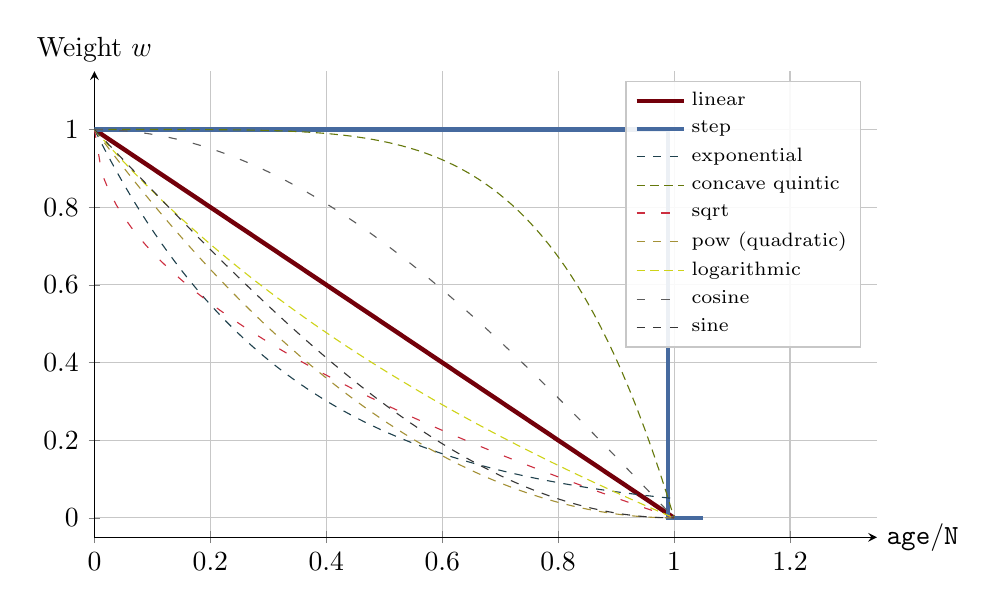
\begin{tikzpicture}
        \begin{axis}[
            width=0.95\textwidth,
            height=7.5cm,
            xlabel={$\texttt{age} / \texttt{N}$},
            ylabel={Weight $w$},
            xmin=0, xmax=1.35,
            ymin=-0.05, ymax=1.15,
            grid=major,
            grid style={ThirtyBlack, thin},
            axis lines=left,
            every axis x label/.style={at={(ticklabel* cs:1.0)}, anchor=west},
            every axis y label/.style={at={(ticklabel* cs:1.0)}, anchor=south},
            legend style={
                at={(0.98,0.98)},
                anchor=north east,
                font=\scriptsize,
                draw=ThirtyBlack,
                fill=white,
                fill opacity=0.9,
                text opacity=1,
            },
            legend cell align=left,
        ]
            % === Built-in modes (solid, ultra thick) ===
            % Linear: w = max(0, 1 - x)
            \addplot[Garnet, ultra thick, solid, domain=0:1, samples=50]
                {max(0, 1-x)};
            \addlegendentry{linear}

            % Step: w = 1 for x<1, 0 at x=1
            \addplot[Atlantic, ultra thick, solid]
                coordinates {(0,1) (0.99,1) (0.99,0) (1.05,0)};
            \addlegendentry{step}

            % === Expression modes (thin, dashed variations) ===
            % Exponential: exp(-x / (1/3)) = exp(-3x)
            \addplot[Congaree, thin, dashed, domain=0:1, samples=80]
                {exp(-x / max(1/3, 0.01))};
            \addlegendentry{exponential}

            % Concave quintic: max(0, 1 - x^5)
            \addplot[Horseshoe, thin, densely dashed, domain=0:1, samples=80]
                {max(0, 1 - x^5)};
            \addlegendentry{concave quintic}

            % Sqrt: 1 - sqrt(x)
            \addplot[Rose, thin, loosely dashed, domain=0:1, samples=80]
                {max(0, 1 - sqrt(x))};
            \addlegendentry{sqrt}

            % Power (quadratic): (1-x)^2
            \addplot[Honeycomb, thin, dashed, domain=0:1, samples=80]
                {(1-x)^2};
            \addlegendentry{pow (quadratic)}

            % Logarithmic: 1 - ln(1 + x*(e-1)) / ln(e)
            \addplot[Grass, thin, densely dashed, domain=0:1, samples=80]
                {max(0, 1 - ln(1 + x*(2.718-1))/ln(2.718))};
            \addlegendentry{logarithmic}

            % Cosine: cos(x * pi/2)
            \addplot[SeventyBlack, thin, loosely dashed, domain=0:1, samples=80]
                {cos(deg(x * pi / 2))};
            \addlegendentry{cosine}

            % Sine: 1 - sin(x * pi/2)
            \addplot[NinetyBlack, thin, dashed, domain=0:1, samples=80]
                {1 - sin(deg(x * pi / 2))};
            \addlegendentry{sine}
        \end{axis}
    \end{tikzpicture}
\end{document}
